\section{Case studies}\label{case-studies}\label{sec:cases}

We present four cases (Table 5.1). Each is a starting point for questions about the decision it models, and Section
7.2 lists the questions we consider open. The cases show how the counterpart changes measured value and how a shortfall divides
into typed action classes. We also reimplemented three counterpart families of an external benchmark, TERMS-Bench, as
an AERead family. Its pre-registered reproduction stopped at its first check, so we report it in Appendix E.10 as
work in progress. We describe all four cases here and specify them in Appendices A--D. Refund
reports compliance with a written policy rather than monetary value.
Each case is a family rather than a fixed task set. It consists of a generator of worlds; a case-specific reference,
which is either a policy that uses only what the deciding side may know or an explicitly labelled full-information
upper bound; an inclusion criterion that keeps the worlds in which the decision matters (its form varies by case;
Appendix E.2); and a set of verifiers. The references differ in what a shortfall means. Against a reachable policy,
the shortfall is the value that a feasible strategy would have kept. Against the best policy given the decider's
information, it is the whole cost of the decisions. Against a full-information bound, it also includes the value of
information that no seat had (Appendix C).

We choose cases by the economic value of the decision rather than by occupation \citep{li2026activities}. An activity qualifies when its
value is decided rather than produced, when a counterparty has its own interest and private information, and when the
result can be scored within a world against a computed reference. The four examples lie in two of the five
transaction classes introduced in §3, business and household purchases. We chose them to span the kinds of verifier
and counterpart, not to sample a representative distribution.

\renewcommand{\thetable}{5.1}
\begin{longtable}[]{@{}
  >{\raggedright\arraybackslash}p{(\linewidth - 8\tabcolsep) * \real{0.2000}}
  >{\raggedright\arraybackslash}p{(\linewidth - 8\tabcolsep) * \real{0.2000}}
  >{\raggedright\arraybackslash}p{(\linewidth - 8\tabcolsep) * \real{0.2000}}
  >{\raggedright\arraybackslash}p{(\linewidth - 8\tabcolsep) * \real{0.2000}}
  >{\raggedright\arraybackslash}p{(\linewidth - 8\tabcolsep) * \real{0.2000}}@{}}
\caption{\textbf{The four cases. Each case is scored in its own units against the reference given in the last column.}}\label{tab:5.1}\tabularnewline
\toprule\noalign{}
\begin{minipage}[b]{\linewidth}\raggedright
Case
\end{minipage} & \begin{minipage}[b]{\linewidth}\raggedright
Real setting
\end{minipage} & \begin{minipage}[b]{\linewidth}\raggedright
What the agent decides
\end{minipage} & \begin{minipage}[b]{\linewidth}\raggedright
Who it faces
\end{minipage} & \begin{minipage}[b]{\linewidth}\raggedright
Scored against
\end{minipage} \\
\midrule\noalign{}
\endhead
\bottomrule\noalign{}
\endlastfoot
Housing & informal rental listings & which listing to inspect, what to offer, and whether to sign when some listings are lemons & scripted landlords; other tenants take listings it leaves & a scripted tenant that uses only what the tenant knows \\
Procurement & wholesale sourcing & pay more for an established supplier, or test a cheaper newcomer, before a deadline & scripted suppliers & the best plan given what the buyer knows, solved exactly \\
Data center & AI-infrastructure contracting & which risk clauses to change, what price to name, and when to sign or walk away & the other side: a script, another model or the same model & the best agreement at both sides' true costs, which neither side knows \\
Refund & customer refund claims & what to ask, disclose, decide and execute under a written policy & three fixed scripted seats; one evaluated seat at a time & the authored policy and protocol, not a monetary optimum \\
\end{longtable}

For the three monetary cases, we report how much room each case leaves as a share of that case's own reference
value. Tables 5.2 to 5.4 give each subject's result and gap in this form. Refund instead reports compliance rates.
Figure 5.2 divides the shortfall by action class in each case's own units. The
cases rely on four kinds of check: an answer key, stated rules, the value of the best policy or a bound, and relative
standing against another agent. None uses a rubric. Every score
is computed by code, with no model in the loop. The kernel's replay recomputes each receipt's own score from its
sealed events, whereas the headline measures of Housing and Procurement are computed by case code outside that
certificate (Appendix F.2). Table E.1 lists every check.

\subsection{Results}\label{results}

The four cases are worked examples that we built and maintain. Their results therefore compare the named agents on
these worlds; they are not qualified benchmark scores. Each result is also bounded by its case's quality-control
gates, which Section 6 describes and Table 6.1 summarises. Below, ``pre-registered'' describes how a comparison was run:
its analysis was committed to the repository before any episode. Sol 6.1 and Opus 5.5 ran through their vendors'
command-line tools rather than our harness. Their results therefore describe agent configurations, meaning the model
with the tool's own instructions and internal turns, at low reasoning effort and without a seed, and the tables mark
them ‡.

\textbf{Housing.} The structure follows informal rental markets on social platforms such as RedNote. Listings are posted
with photos that a tenant cannot check before viewing, a viewing costs time, and good listings are often taken while
the tenant decides. We set the rents, the lemon share and the inspection cost ourselves; they are not drawn from
platform data. A tenant chooses among four listings, two of which are lemons. It knows its own value v\_ℓ for each
listing if sound, but not which two are lemons; each of the six pairs is equally likely. In each of three rounds it
may pay \$25 to inspect one listing, make one offer, and sign or walk away from a lease it is offered, while each
listing it did not bid on is taken by outside demand with probability ½. Signing listing ℓ at rent x after k
inspections pays

\[ \text{v\textsubscript{ℓ} − 1,000·𝟙[ℓ is a lemon] − x − 25k,} \tag{1} \]

and signing nothing pays −25k. The difficulty lies in information. A listing worth \$400 more than its ask if sound is
worth 400 − ½·1,000 = −\$100 if signed blind at the ask, but ½·400 − 25 = +\$175 if it is inspected first and signed only
when sound; inspecting a second listing takes another round, in which each listing not bid on may be taken. A
landlord's reply can reveal a lemon at no cost: every world is played against one landlord kind whose reply to a low
offer reveals a lemon and one whose reply does not. The revealing (leaky) landlord prices a lemon from its own cost,
which is lower than a sound listing's by exactly the amount the lemon costs the tenant, so once its quality is known
a lemon at that price is as good a lease as the same listing sound, to within \$5. We score a blind signing at its expected value given what the
tenant knew, so that the score follows the decision rather than the draw, with the odds conditioned on every
informative landlord reply. This paper introduces the corrected measure. The comparison reported here, v15, was pre-registered before any of
its artifacts. Each included world is screened so that the best informed tenant beats a simple inspect-then-sign rule
by at least \$25, and the tenant's task prompt states how landlords price. A holdout of 40 worlds changes one
mechanism, outside demand at 0.3 a round, and its task prompt says so.

\renewcommand{\thetable}{5.2}
\begin{longtable}[]{@{}
  >{\raggedright\arraybackslash}p{(\linewidth - 8\tabcolsep) * \real{0.1579}}
  >{\raggedleft\arraybackslash}p{(\linewidth - 8\tabcolsep) * \real{0.2105}}
  >{\raggedleft\arraybackslash}p{(\linewidth - 8\tabcolsep) * \real{0.2105}}
  >{\raggedleft\arraybackslash}p{(\linewidth - 8\tabcolsep) * \real{0.2105}}
  >{\raggedleft\arraybackslash}p{(\linewidth - 8\tabcolsep) * \real{0.2105}}@{}}
\caption{\textbf{Housing v15, main evaluation set (260 worlds; 200 with the favourite a lemon, 60 sound): each model's mean net payoff under the corrected measure, averaged over the two landlord arms, divided by the best informed tenant's mean (\$307 a world; each stratum and the holdout by their own). Differences are mean dollar contrasts over worlds on the same scale, in percentage points, with 95\% intervals. ‡ Agent configuration (command-line tool, low reasoning effort, no seed).}}\label{tab:5.2}\tabularnewline
\toprule\noalign{}
\begin{minipage}[b]{\linewidth}\raggedright
\end{minipage} & \begin{minipage}[b]{\linewidth}\raggedleft
Gemini 3.8 Flash
\end{minipage} & \begin{minipage}[b]{\linewidth}\raggedleft
GPT-6 Luna
\end{minipage} & \begin{minipage}[b]{\linewidth}\raggedleft
Sol 6.1 (Codex)‡, addendum
\end{minipage} & \begin{minipage}[b]{\linewidth}\raggedleft
Opus 5.5 (Claude Code)‡, addendum
\end{minipage} \\
\midrule\noalign{}
\endhead
\bottomrule\noalign{}
\endlastfoot
Share of the best informed tenant's value & 78.7\% & 62.9\% & 90.4\% & 80.4\% \\
Favourite is a lemon / sound & 68.8\% / 100.0\% & 46.8\% / 97.3\% & 85.9\% / 100.0\% & 71.2\% / 100.0\% \\
Minus \texttt{inspect\_\allowbreak{}then\_\allowbreak{}sign} (the pre-registered beatability baseline), points & +29.3 {[}+24.7, +33.8{]} & +13.4 {[}+8.2, +18.6{]} & +40.9 {[}+36.2, +45.6{]} & +30.9 {[}+26.3, +35.5{]} \\
Minus \texttt{inspect\_\allowbreak{}lowball} (v14's reachable reference), points & −16.6 {[}−20.8, −12.5{]} & −32.5 {[}−37.8, −27.3{]} & −5.0 {[}−8.0, −2.0{]} & −15.0 {[}−18.9, −11.0{]} \\
Holdout (40 worlds, outside demand at 0.3) & 79.3\% & 61.1\% & 88.0\% & 80.1\% \\
\end{longtable}

Both pre-registered models beat the pre-registered baseline and stay below the best informed tenant, and almost all
of their shortfall arises in worlds whose favourite listing is a lemon. Gemini leads Luna by 15.9 points {[}11.3, 20.4{]}
of the best informed tenant's value. This lead is significant under the pre-registered analysis. Its lower end,
however, falls below 16.3 points, the share that corresponds to the \$50 we pre-registered as the smallest meaningful
difference, so the lead is not shown to exceed that band. Where the favourite is a lemon, Gemini keeps 69\% and Luna
47\% of the best informed tenant's value; where it is sound, they keep 100\% and 97\%. Both models also stay below
\texttt{inspect\_\allowbreak{}lowball}, a simple rule that inspects the favourite and opens with the lowest possible offer, which earns
95.4\% of the best informed tenant's value. Most of the shortfall in lemon worlds comes from one choice: declining a
known lemon that the leaky landlord prices to be exactly as good as the same listing sound (Section 5.2). That
equality is a knife-edge feature of our design, not of lemons markets in general (Section 7). The holdout points the
same way (Table 5.2, last row).

\textbf{Further runs.} v15 differs from the earlier v14 comparison in four ways at once (the screened evaluation set, the
stated pricing rule, the corrected measure as primary, and receipts that score the deciding tenant). Its levels are
therefore not comparable with v14's, and we attribute no change between them to the models or to any single
difference; Appendix E.4 reports v14. Two pre-registered addenda ran outside v15's contrasts. In the first, GLM 5.3
Flash, which was excluded at the pre-run profile check because its provider had changed quantization, ran on a
provider that serves v14's quantization; it does not beat \texttt{inspect\_\allowbreak{}then\_\allowbreak{}sign}. In the second, Sol 6.1 and Opus 5.5
played through their command-line tools. Sol keeps the largest share of any model, and Opus cannot be distinguished
from Gemini. Appendix E.4 gives the addenda's contrasts, the A/A arm, which shows that run-to-run noise is well inside the \$50 band, and the holdout.

\textbf{Procurement.} The structure follows wholesale sourcing on B2B platforms such as Alibaba's 1688. A displayed price
is not a quote, a listing's quality is known only after it is checked, and new sellers of one kind often buy from the
same factory. A buyer owes 50 kits by a deadline and awards the order to one supplier: either a recorded supplier with
a long clean record or one of three newcomers. Each newcomer is good, late or poor. The buyer knows only the odds,
which are read from the record of the newcomer's seller kind, and that newcomers of one kind share a source with a
stated probability (0.5 to 0.95), in which case they are all of the same type. Two features follow our own sourcing on
1688. A newcomer's price relative to the recorded supplier's is drawn from the price gaps in that record, so a
newcomer is dearer about half the time, and a newcomer answers a quote request only a third of the time. We set the
case's other quantities ourselves. Among up to ten actions the buyer may request a quote (\$2 and a day; an answered
quote exposes a late supplier), request a sample (\$20 to \$240 and three days; it always arrives and exposes a poor
supplier), look up a listing's registered factory (\$1; two lookups in one kind show whether the kind shares a
source), award the order, or defer. An award that delivers k kits on time earns

\[ \text{37k − 12(50 − k) − cost of the order − cost of the information bought,} \tag{2} \]

and an award that delivers fewer than 40 kits, as a late or poor supplier does, earns −\$600 less the information
bought (Appendix A.2).

The difficulty is a test worth taking only for what it reveals about another supplier. Every world in the evaluation
set is one in which a rule that plans a single newcomer's test exactly (what to request first, how often to repeat an
unanswered quote, and when to give up) pays the premium, while the best policy acts on a newcomer first (a quote
request in 14 worlds, a factory lookup in 6) and beats paying the premium by at least 10\%. Such worlds are a selected
tail: 20 of the 5,164 seeds we generated (0.4\%) pass the inclusion criterion, so the results describe worlds of this
kind, not the generator's typical world. In one world the recorded supplier asks \$24.95. A newcomer asks \$12.47, but its sample
costs \$200 and its odds are 0.20 good, 0.15 late and 0.65 poor, so testing it on its own loses money. A second
newcomer of the same seller kind asks \$26.87, more than the recorded supplier, so it is never worth buying; but its
sample costs \$30, and the two share a source with probability 0.95. Once the cheap newcomer's quote has come back
clean, a sound sample of the dear newcomer raises the cheap newcomer's probability of being good to 0.94, and a poor
sample lowers it to 0.01. The best policy therefore requests a quote from the cheap newcomer; if the quote comes back
clean, it samples the dear newcomer, looks both up, and only then pays for the \$200 sample. It earns 11.8\% more than
paying the premium. Every action is charged the value it gave up relative to the exact best informed policy at that
point.

\renewcommand{\thetable}{5.3}
\begin{longtable}[]{@{}
  >{\raggedright\arraybackslash}p{(\linewidth - 6\tabcolsep) * \real{0.2000}}
  >{\raggedleft\arraybackslash}p{(\linewidth - 6\tabcolsep) * \real{0.2667}}
  >{\raggedleft\arraybackslash}p{(\linewidth - 6\tabcolsep) * \real{0.2667}}
  >{\raggedleft\arraybackslash}p{(\linewidth - 6\tabcolsep) * \real{0.2667}}@{}}
\caption{\textbf{Procurement, the 20 pre-registered worlds, two plays each: the share of the gap between paying the premium and the best policy that each model closes (a mean over worlds, with 95\% t intervals), the loss per world relative to the best policy, and the plays that touched a newcomer. The one-step rule's 0\% holds by construction of the inclusion criterion. ‡ Agent configuration (command-line tool, low reasoning effort, no seed).}}\label{tab:5.3}\tabularnewline
\toprule\noalign{}
\begin{minipage}[b]{\linewidth}\raggedright
\end{minipage} & \begin{minipage}[b]{\linewidth}\raggedleft
Share of the gap closed
\end{minipage} & \begin{minipage}[b]{\linewidth}\raggedleft
Loss per world
\end{minipage} & \begin{minipage}[b]{\linewidth}\raggedleft
Plays touching a newcomer
\end{minipage} \\
\midrule\noalign{}
\endhead
\bottomrule\noalign{}
\endlastfoot
Sol 6.1 (Codex)‡ & 35\% {[}18, 52{]}, p = 0.0003 & \$32.51 & 26 of 40 \\
Opus 5.5 (Claude Code)‡ & 0\% in every world & \$51.25 & 0 of 40 \\
Gemini 3.8 Flash & 0\% in every world & \$51.25 & 0 of 40 \\
GPT-6 Luna & −14\% {[}−21, −7{]} & \$58.10 & 0 of 40 \\
\emph{Exact rules on the same worlds} & & & \\
Paying the premium; a rule that plans one newcomer's test & 0\% & \$51.25 & \\
Shortcut: sample the newcomer with the cheapest sample first, ignoring seller kinds & 33\% & \$33.46 & \\
A rule that may test two newcomers & 82\% & \$8.38 & \\
\end{longtable}

\begin{figure}[htbp]\centering\renewcommand{\thefigure}{5.1}
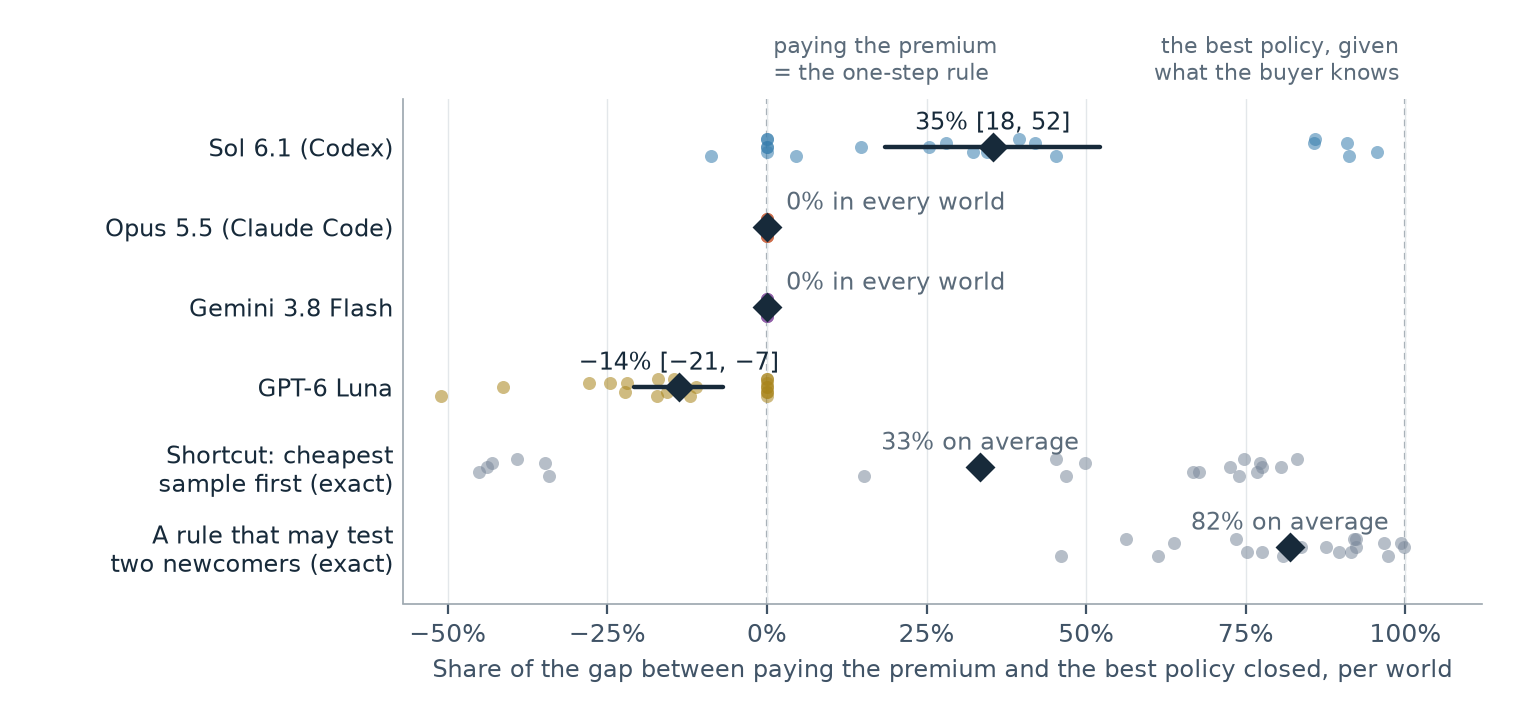
\includegraphics[width=\linewidth]{figures/procurement_v3_gap_closed.png}
\caption{\textbf{Procurement, the 20 pre-registered worlds: the share of the gap between paying the premium and the best policy closed, world by world.} Each dot is
one world, the mean of its two plays; diamonds are means, bars are 95\% t intervals, and the gray rows are exact rules.}
\label{fig:5.1}
\end{figure}

The pre-registered test asks whether Sol 6.1 closes any of this gap. A rule that plans one newcomer's test exactly
closes none by construction, because the inclusion criterion keeps only worlds in which it pays the premium. Sol
closes 35\% (95\% t interval 18--52\%, p = 0.0003). The worlds were drawn, and this test pre-registered, before any play, and the claim concerns Sol
alone. Sol's play varies by world (Figure 5.1): it closes most of the gap in some worlds and none in others. The
other three models never touched a newcomer and paid the premium. Luna falls below paying the premium because it
ordered 50 units where 55 was best in 15 of its 40 plays. A shortcut that ignores seller kinds and first samples the
newcomer whose sample is cheapest closes 33\%, about Sol's share. Sol does not play that shortcut, however; its tests
follow price. A rule allowed to test two newcomers closes 82\%, so the remaining headroom lies in planning one test
beyond the one in hand.

\textbf{Further runs.} A development pilot and four diagnostics on this evaluation set, among them a frozen
control, leave this picture unchanged (Appendix E.4, Table E.15). One of them bears on why Opus never tests. Asked,
with no play, how a sample of one newcomer changes the odds of another of its kind, Opus answered all 18 questions
within 0.05 of the exact value, as Sol did. Opus therefore applies the sharing rule when asked, but does not plan with
it. On an earlier evaluation set, in which quotes always arrive and newcomers never share a source, a rule that looks
one test ahead comes within 0.01\% of the best policy, so that set cannot separate the models (Appendix E.4).

\textbf{Data center.} The structure follows a real AI-infrastructure engagement in which a system integrator bundles
hardware, data-center space, staffing and software into a working system for a client. Hardware can arrive late or
defective, the site may not be ready, and the contract's warranty, delay-damages, liability-cap, site-readiness,
deposit and burn-in clauses decide who bears each cost. We set the costs, probabilities and prices ourselves. Client
and integrator negotiate one agreement, consisting of a position on each of the eight clauses (600 distinct
agreements) and an all-in price p.~Each side knows its own cost of carrying risk and only the probability distribution
of the other's: the integrator's pre-staging cost and risk charge, and the client's risk charge. Over six alternating
moves, a side may redline any clauses and name a price, sign the standing version, or walk away, and each redline
after the first move costs \$25k. In thousands of dollars and net of redline fees, a signed agreement c pays the
integrator and the client, respectively,

\[ \text{π\textsubscript{I} = p − C\textsubscript{I}(c) − 500,  π\textsubscript{C} = O\textsubscript{C} − p − C\textsubscript{C}(c),} \tag{3} \]

where 500 is the integrator's outside option, O\_C the client's, and C\_I and C\_C each side's expected cost of the risks
that the clauses leave with it, marked up by its risk charge; no deal pays only the fees. The difficulty is that price
only divides the value, while the clauses determine how much value there is, and the best clauses depend on what the
other side hides. Burn-in, for example, costs the integrator \$40k and, in one world, costs the client a week's delay
worth \$110k, and it halves the probability of a \$3 million incident that the client carries. It therefore lowers joint
cost by \$41k for a client with the highest risk charge and raises it by \$19k or \$64k for the other two, and the
integrator cannot tell which client it faces. The comparison reported here (v2) was pre-registered before its runs, on
80 included worlds (from 5,436 scanned), 72 of them with a mutually beneficial deal. Both command-line tools were
isolated, the client's task prompt states its walk-away point, and a world is included only if the integrator has at
least \$25k of room over a price-only rule.

\textbf{What v2 tests.} Against the fixed scripted client, the integrator seat tests bargaining over clauses and price, not
inference about the other side. The client's risk charge is drawn in every world, but the scripted client's first
reply reveals it, so knowing the client's type is worth less than 1\% of the value available to the best informed
integrator. The burn-in example above describes the case's design, which v2's counterpart does not exercise.

\renewcommand{\thetable}{5.4}
\begin{longtable}[]{@{}
  >{\raggedright\arraybackslash}p{(\linewidth - 6\tabcolsep) * \real{0.2143}}
  >{\raggedleft\arraybackslash}p{(\linewidth - 6\tabcolsep) * \real{0.2857}}
  >{\raggedright\arraybackslash}p{(\linewidth - 6\tabcolsep) * \real{0.2143}}
  >{\raggedleft\arraybackslash}p{(\linewidth - 6\tabcolsep) * \real{0.2857}}@{}}
\caption{\textbf{Data center v2, Sol 6.1 (Codex) against Opus 5.5 (Claude Code) on the 72 deal worlds.} Pre-registered
contrasts in a seat's earnings above its outside option at true costs, in points of the value available in a deal
(\$309k a world), with 95\% intervals and Holm correction. The head-to-head row counts a transfer between the agents twice.
Both agents are agent configurations (command-line tool, low reasoning effort, no seed).}\label{tab:5.4}\tabularnewline
\toprule\noalign{}
\begin{minipage}[b]{\linewidth}\raggedright
Primary contrast
\end{minipage} & \begin{minipage}[b]{\linewidth}\raggedleft
Worlds
\end{minipage} & \begin{minipage}[b]{\linewidth}\raggedright
Estimate {[}95\% interval{]}
\end{minipage} & \begin{minipage}[b]{\linewidth}\raggedleft
Holm p
\end{minipage} \\
\midrule\noalign{}
\endhead
\bottomrule\noalign{}
\endlastfoot
Head to head: Sol minus Opus earnings, seat-averaged & 72 deal & +41.7 {[}31.3, 52.0{]} & 6.1e-11 \\
Integrator against the firm client: Sol minus Opus & 72 deal & +7.5 {[}1.8, 13.2{]} & 0.022 \\
Sol as integrator minus the price-only rule & 72 deal & +7.3 {[}2.6, 12.0{]} & 0.008 \\
Opus as integrator minus the price-only rule & 72 deal & −0.2 {[}−5.5, 5.2{]} & 0.95 \\
\end{longtable}

The counterpart changes the measured gap. Head to head, Sol's earnings exceed Opus's by 41.7 points of the value
available, and against the same scripted firm client by 7.5 points (Table 5.4). Both gaps are significant under the
Holm correction, and neither is shown to reach its pre-registered minimum. The two numbers are not on one scale. Head
to head, a dollar that Sol takes from Opus raises Sol's earnings and lowers Opus's, so it counts twice in the
difference; against the script, a dollar that Sol gains leaves Opus's earnings unchanged. Counting each transfer between the two agents once halves the head-to-head gap to 20.8 points {[}15.7, 26.0{]}, and
this is the number we compare with the script. Against the script we use the pre-registered integrator-seat gap,
7.5 points, rather than an average over both seats (4.1 points, Appendix E.4), because the client seat separates
nothing against the script, as shown below; using 7.5 makes the comparison conservative. The head-to-head gap is
therefore about three times the script gap, and the paired difference, which we computed after the runs, is 13.4
points {[}6.4, 20.3{]}. As
integrator, Sol beats the price-only rule, and Opus earns what the rule earns. As client, with its walk-away point
stated, neither model signs below that point, and the client seat separates nothing. After both runs we computed the
best informed turn-by-turn policy against the same scripted client (Appendix C.3). Sol captures about 20\% of the room
between the price-only rule and that policy.

\textbf{Further runs.} An earlier pre-registered comparison (v1) ran without isolated command-line tools, without the
client's walk-away point in its task prompt, and without the inclusion screen against the price-only rule. Appendix
E.4 reports it, with the development results and the figures behind this paragraph.

\textbf{Refund.} A refund is more than a choice between approving and denying a claim. The intake desk must ask for the
facts that decide it, the customer must disclose the requested records, the policy seat must apply the rules in their
stated order, and the payments seat must execute the confirmed obligation exactly once. A correct outcome proposed
before the evidence arrives is therefore not a correct decision, and a payment that follows a wrong proposal is not a
correct payment. The score is compliance with an authored policy, not money recovered or business value; a refund
amount is a field to verify, not a welfare measure. A world combines a product category (perishable goods,
electronics, software or apparel) with an interaction rule, such as conflicting identity records, a pending payment
or an evidence threshold. The public policy states the precedence of its rules, which facts each branch requires, the
allowed outcomes and the amount formulae. The customer holds the private facts, and no evaluated seat sees the answer
key. Each world comes as a counterfactual pair that changes the stated facts and keeps the rest of the world fixed.
Appendix A.4 specifies the case.

We evaluate one seat at a time while the other three follow fixed scripts. The comparison reported here is an
amended, sequential developmental calibration, not a pre-registered comparison. Gemini 2.5 Flash Lite, Gemini 2.5
Pro and GPT-6-sol each played a frozen selection of 66 seat-specific pair templates, both variants twice, for 792
episodes in all. The score is weighted strict trajectory compliance: the evaluated seat's decisions and its
protocol obligations must all hold in the same episode, and episodes are weighted as Appendix E.4 gives.

Flash Lite separates from the two stronger models in three of the four seats. It reaches 38.3\% weighted strict compliance
as intake, 33.3\% as policy and 35.6\% as payments, while Gemini 2.5 Pro and GPT-6-sol reach at least 98.6\% in every
seat. Pro's lead over Flash Lite in those seats, 60.8 to 65.3 percentage points, remains significant after Holm
adjustment across the eight frozen contrasts. Above Flash Lite the panel is saturated: both stronger models pass 62
of the 66 templates on both variants in both repetitions, and every model passes every customer episode. The panel
therefore cannot rank the stronger models, and no contrast between them is evidence that they are equivalent.
Figure E.1 in Appendix E.4 shows every seat and diagnostic.

\textbf{Further runs.} A later public release of the environment adds customer and intake panels. Its 1,072 scripted
trajectories on the current runtime pass with full scores, which establishes the environment's conformance, not model
performance. The calibration's model episodes ran on an earlier, versioned runner and were audited there; porting the
environment to the current runtime does not turn them into results on the current kernel (Appendix H). A separate
redesign, Refund V3, is not part of these results. Appendix E.4 gives the weights, the eight contrasts and the
failure checks.

\subsection{Where the shortfall comes from}\label{where-the-shortfall-comes-from}

Figure 5.2 divides each case's shortfall into observed action classes. The components sum to the total under a stated
priority order, and they describe what happened, not its cause. The Housing panel shows v15's two pre-registered
models and three addendum agents (A: GLM; B: Sol and Opus through their command-line tools), measured below the
reachable rule \texttt{inspect\_\allowbreak{}lowball}. Negative components, at most \$0.4 a world, are not drawn. The Data center panel
shows v2's joint loss relative to the full-information bound against the firm counterparts, with each redline after
the first move charged \$25k, across all 80 worlds with both seats averaged. The Refund panel shows the policy seat of
the V2.5 calibration, 72 episodes per model, in percentage points of strict compliance; each failed episode is
counted once, under the first applicable class. Appendix E.5 gives the classification
rules and full subject tables, Appendix E.7 the Data-center breakdown and its uncertainty, and Tables 5.3, E.9 and
E.10 the intervals and exact values.

\begin{figure}[htbp]\centering\renewcommand{\thefigure}{5.2}
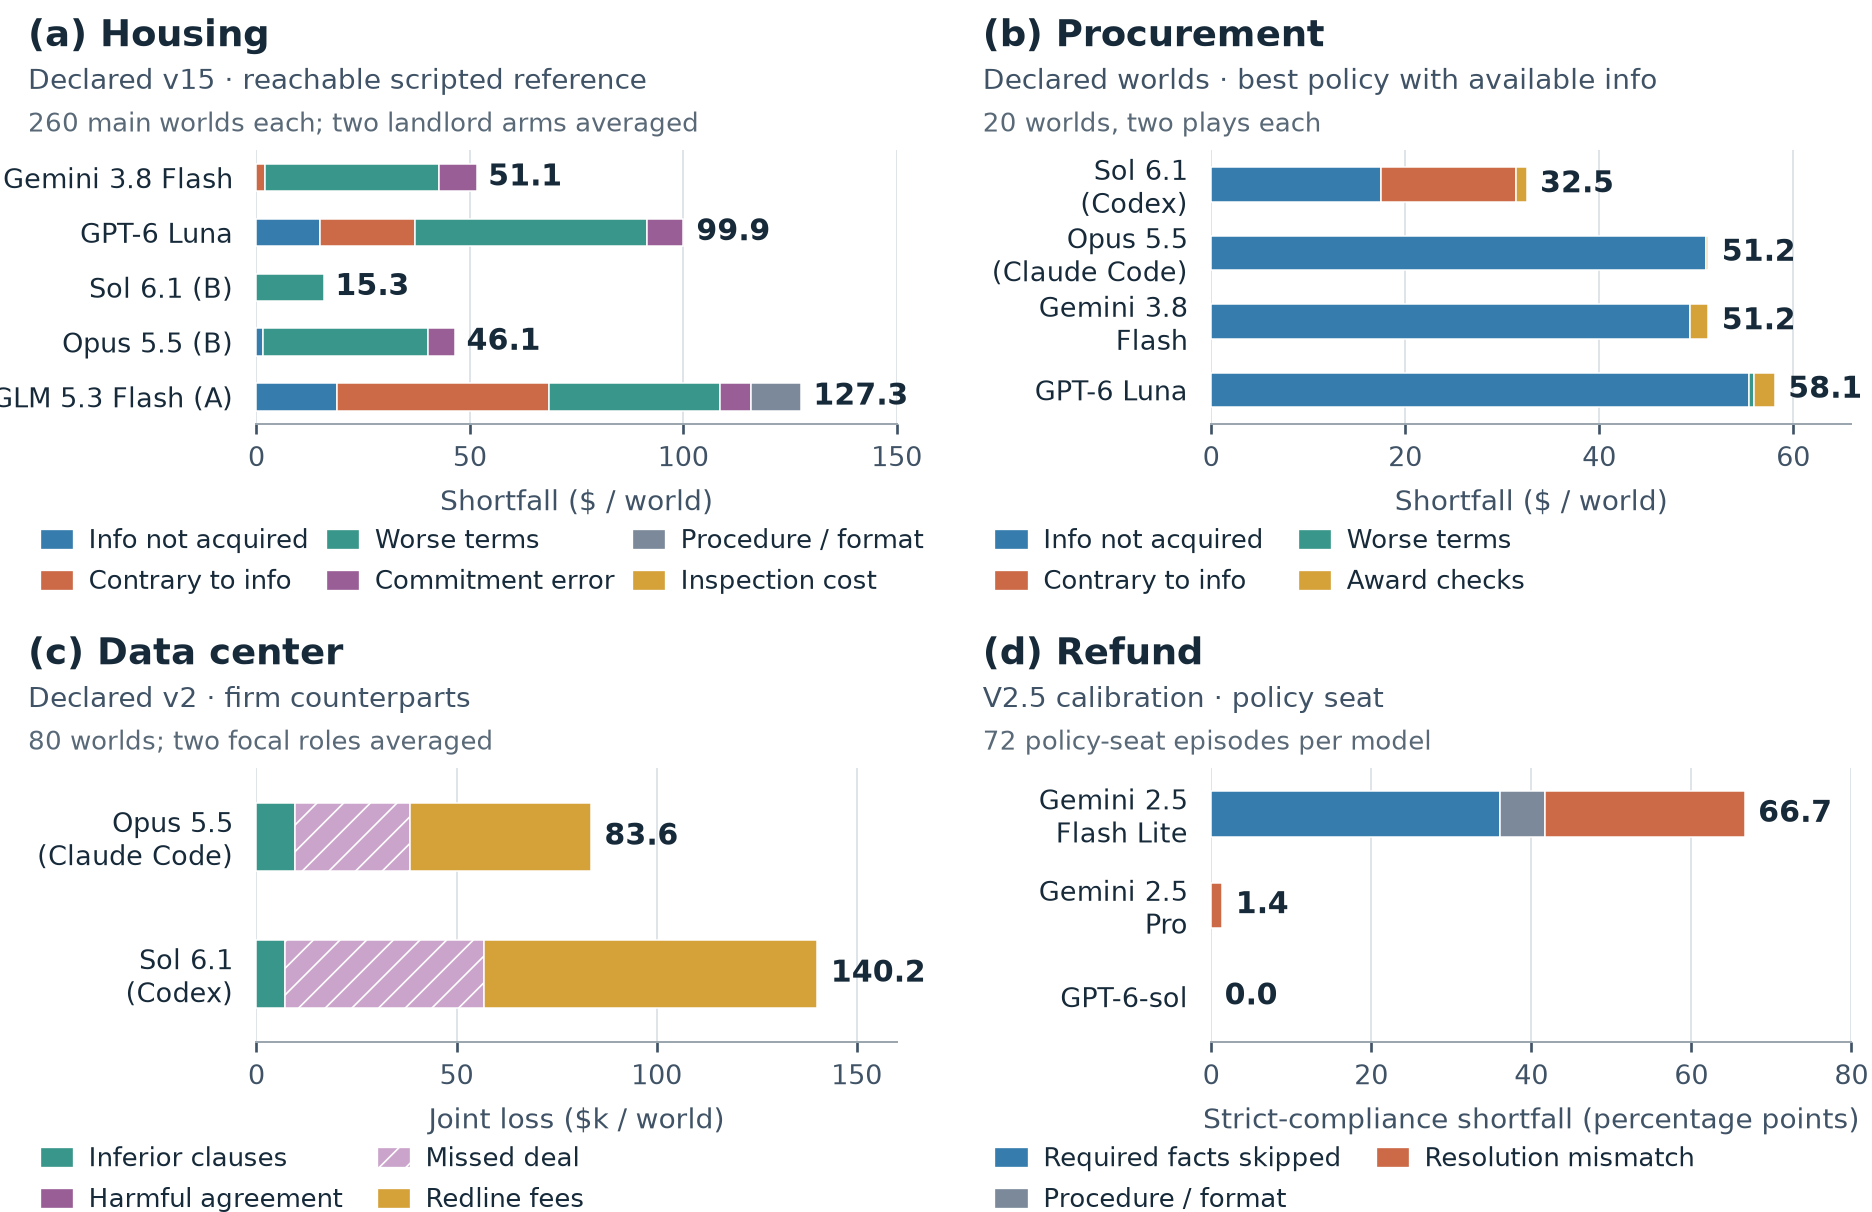
\includegraphics[width=\linewidth]{figures/shortfall_by_case.png}
\caption{\textbf{Shortfall to each case's reference, divided by observed action class.} Labels give mean totals (lower
is better); each panel has its own reference, units and scale. Housing uses the 260 main worlds of Table 5.2,
Procurement the 20 worlds of Table 5.3, Data center the 80 worlds of Table 5.4, and Refund the 72 policy-seat
episodes per model of the calibration (Appendix E.4).}
\label{fig:5.2}
\end{figure}

The labels name what happened. The mechanism behind each large segment is as follows.

\textbf{Procurement: three models never test, and Sol secures the recorded supplier first.} Opus, Gemini and Luna asked
no newcomer for anything in any of their 120 plays: they requested quotes and samples from the recorded supplier and
awarded it the order, so nearly all of their loss is information not acquired, and the rest is award checks, each of
which spends an action. Luna loses \$6.85 a world more than paying the premium (\$58.10 against \$51.25 in Table 5.3), all of it from
ordering 50 units where 55 was best in 15 of its 40 plays. The pre-registered classes file an award's whole loss under
information not acquired when the award came before a worthwhile test. Most of this quantity loss therefore appears
in Luna's information-not-acquired segment of Figure 5.2 rather than under worse terms; Appendix E.5 gives the split. Sol's loss divides by
world. Where it never tested a newcomer that the best policy would have tested, it lost \$17.5 a world. Where it did
test, it often first requested a quote and a sample from the recorded supplier, spending days and actions before the
newcomer test that the stated odds and clock made best (\$8.9 a world), or it awarded the order while a newcomer test
it had begun was still worth finishing (\$3.2).

\textbf{Housing, Gemini: it drops a known lemon even where the lemon is the better lease.} Worse terms account for 80\% of
its shortfall relative to the reachable rule (\$40.7 of \$51.1 a world), and nearly all of it comes from one move. Under
the landlord kind that prices a lemon from its own lower cost, a lemon's landlord counters about \$1,000 below a sound
listing's floor (\$995 to \$1,000 in these worlds), so a known lemon signed at that counter is worth what the listing
would be worth sound at a sound floor. This holds exactly in 187 of the 200 worlds whose favourite is a lemon, and
within \$5 in the rest. The equality is a property of our design: the leaky landlord passes the whole of a lemon's
discount through to its rent. The rule inspects the favourite, finds the lemon, offers \$0 and signs the counter in all 200.
Gemini also inspected the favourite and found the lemon in all 200, but made an offer on it in only 4; in 172 episodes
it leased a sound listing that left it with less (\$65.0 a world). Under the other landlord kind the rule leases nothing
in 77 worlds, and Gemini's leases there offset \$26.5 a world. Gemini does read landlords' replies: of 74 replies that
proved a lemon, it walked away from 64 and signed above the lemon's value once. Ending with no lease where the rule
leased costs a further \$8.9 (12 of 520 episodes). Within the case's stated rules, declining such a lemon is an error, because
the task prompt states how landlords price; in a market where the discount is smaller than the loss, the same choice
could be right. The \$65.0 a world from these leases alone exceeds Gemini's whole worse-terms class, which its leases
under the pooled kind partly offset, so most of Gemini's measured shortfall rests on full pass-through.

\textbf{Housing, Luna: it drops the lemons worth taking and signs ones that cost it.} Its shortfall relative to the
reachable rule is \$99.9 a world. Worse terms (54\%, \$54.3) follow Gemini's pattern and rest on the same full pass-through: in the same 200 worlds Luna found
the lemon favourite in 197 and made an offer on it in 7, and in 154 episodes it leased a sound listing that left it
with less (\$57.7 a world). Signing a listing that a landlord's reply had proved a lemon accounts for 22\% (\$22.2,
11 episodes): the landlord accepted Luna's offer at a rent that no sound landlord would take, which by the stated
pricing rule proves a lemon, and Luna signed at that rent, above the lemon's value. Of 89 such replies, it walked away
from 58 and signed 20 at or below the lemon's value. Another 15\% (\$14.9, 64 episodes) comes from signing without
settling quality under the landlord kind whose replies reveal nothing, where an inspection was worth its \$25 fee every
time; 21 of those listings were lemons. Ending with no lease where the rule leased costs \$8.6. In v14, whose task
prompt did not state how landlords price, the reply-proved lemon accounted for 60\% of Luna's shortfall.

\textbf{Housing, Sol and Opus (addendum B): what remains is the price.} Neither lost anything by acting against what it
knew, and neither left a worthwhile inspection undone, apart from Opus's \$1.4 a world. Worse terms account for all of
Sol's \$15.3 shortfall (\$15.7, offset by \$0.4 of inspection fees it saved) and for 84\% of Opus's \$46.1 (\$38.8); ending
with no lease where the rule leased costs Opus a further \$6.3.

\textbf{Refund, Flash Lite: a plausible answer is not a complete policy path.} In the policy seat, 26 of its 72 episodes
propose a decision before the required evidence has been collected, including proposals whose stated outcome is
correct. Another 4 end with an invalid request or no scoreable final resolution, and 18 reach a resolution that
does not match the policy, the workflow or the prescribed payment. Counted once each in that order, these classes
account for 36.1, 5.6 and 25.0 points of its 66.7-point shortfall. Pro's 1.4-point shortfall is a single error in the
liability field, and GPT-6-sol has none in this selection. Figure E.1 shows why the diagnostic measures stay beside
strict compliance: Flash Lite passes a third of the individual policy episodes, but in no pair do both variants pass
within a repetition.

\textbf{Data center: fees, then deals the client walked away from.} Every redline after the opening move costs \$25k. The
full-information reference signs the best agreement at once, so each fee counts as loss, whichever side paid it.
Against the firm counterparts, across all 80 worlds with both seats averaged, fees account for 59\% of Sol's joint loss
(\$83.4k of \$140.2k a world) and 54\% of Opus's (\$45.3k of \$83.6k). Sol redlines more: as integrator it made 371
redlines to the firm client's 262, whereas Opus made 227 to 189. Some of those redlines buy better clauses, and a seat
that does not know the other side's costs may need them, so their share alone does not show wasted negotiation. Nearly
all of the remaining loss is deals lost in worlds that had one (35\% of Sol's loss and 34\% of Opus's), and every one of
them ended with the client walking away. With each model as integrator, the firm client walked away from Sol in 40 of
its 144 plays of deal worlds and from Opus in 14. As client, each model walked away in 26 of the 72 deal worlds. No
agreement was harmful: with the walk-away point in the task prompt, neither model signed in any of the 8 worlds
without a deal.

The pre-registered plan included a replay of the recorded moves at other fees, which shows what the same moves would
earn, not how the models would play. Without fees, Sol still loses more joint value than Opus against the firm
counterparts (\$63.1k against \$42.5k a world, seats averaged) and earns more in both seats. At \$50k a redline its
earnings fall below Opus's (as integrator 67.9 against 69.7, as client 1.3 against 22.8, in thousands of dollars per
deal world), because it redlines more. Appendix E.9 gives v1's fuller replay.

\textbf{Across the cases.} Four findings hold across the cases. First, the gap lies in a stratum that the design fixes in
advance, so every case reports by stratum and pools last. Second, the counterpart is part of the measurement, so a
claim names the counterparts it covers. Third, what the task prompt states moves the score as much as the subject does
(stating two rules cut procurement loss by \$11 to \$14; stating a walk-away cost cut losing signatures from 15 of 60 to
1 of 60), so the task prompt is a versioned part of the case. Fourth, a pattern found by looking back is a hypothesis
until a pre-registered test confirms it.
